%%%%%%%%%%%%%%%Conjectures regarding values of Riemann zeta function at Gram Points%%%%%%%%%%%%%%%%%%%%%%%%%%%%%%%%%%%%%%%%%%%%%%%%%%%%%%%%%%%%%
%

\documentclass[twoside]{article}
\usepackage{graphicx}
\usepackage{amsmath,amsthm,amssymb,verbatim}
\usepackage{fancyhdr}
\pagestyle{fancy}
\usepackage{url}

\def\blfootnote{\xdef\@thefnmark{}\@footnotetext} 
\long\def\symbolfootnote[#1]#2{\begingroup%
\def\thefootnote{\fnsymbol{footnote}}\footnote[#1]{#2}\endgroup} 

\newtheorem{mydef}{Conjecture}

\setcounter{page}{1}
\begin{document}

\date{}
\lhead[]{}
\chead[\underline{xxx}]{\it{AMO - Advanced Modeling and Optimization, Volume xx, Number xx, 2017}}
\rhead[]{}

\title{\bf{Conjectures regarding Riemann zeta function at Gram Points}}


\author{O. Shanker 
 \thanks{Mountain View, CA 94041, U. S. A. Email: oshanker@gmail.com
 }
}

\maketitle
\thispagestyle{fancy}

\begin{abstract}
Riemann's hypothesis is one of the key unsolved problems which is attracting
a lot of attention. 
Researchers are making extensive numerical studies of the location of the 
zeta function zeros to complement the theoretical work. 
The evaluation of the zeta function at large heights involves time consuming
calculations. The values of the 
zeta function at Gram Points plays an important role in the computations. In 
this work we present two conjectures about the distribution of zeta values at the 
the Gram Points. We present quantitative evidence for the conjectures.
\end{abstract}


\symbolfootnote[0]{\bf{*AMO - Advanced Modeling and Optimization. ISSN: xxx}}


\clearpage
\chead[\underline{O. Shanker}]{\underline{Conjectures regarding Riemann zeta function at Gram Points}}


\section{Introduction}
Riemann's hypothesis about the location of 
the roots of the Riemann zeta function is a key unsolved problem in mathematics,
which challenges us to this day. The study also has ramifications in physics and
random matrix theory. 
There is an impressive body of empirical evidence for his hypothesis,
but a formal proof has been elusive. The numerical studies have found
regions where the hypothesis is almost violated, but no counter-example has
been found. The numerical evaluation of the zeros is time-consuming, and the values of the 
zeta function at Gram Points plays an important role in the computations~\cite{korolev1,korolev2}. In 
this work we present two conjectures about the distribution of zeta values at the 
the Gram Points. We present quantitative evidence for the conjectures. 
\begin{mydef}\label{antisymmetry}
(even-odd antisymmetry): The distribution of the zeta values for odd gram points is the negative of the distribution of zeta values for the even zeta points.
\end{mydef}
\begin{mydef}\label{symmetry}
(forward-backward symmetry): When we consider a sequence of zeta values at consecutive gram points, the properties of the sequence are symmetric with respect to the direction of the sequence of gram points (i.e., the sequence behaves similarly whether we consider the points in increasing order or in decreasing order).
\end{mydef}

The paper is organized as follows.
Section~\ref{sec2} establishes the required notation for the 
Riemann Zeta Function. 
Section~\ref{sec3} describes the numerical evaluation of the Riemann zeta function. 
Section~\ref{conclusions}
gives a brief summary of the results. 


\section{\label{sec2}Theory of zero distributions of Riemann zeta function }

\begin{figure}
\centering
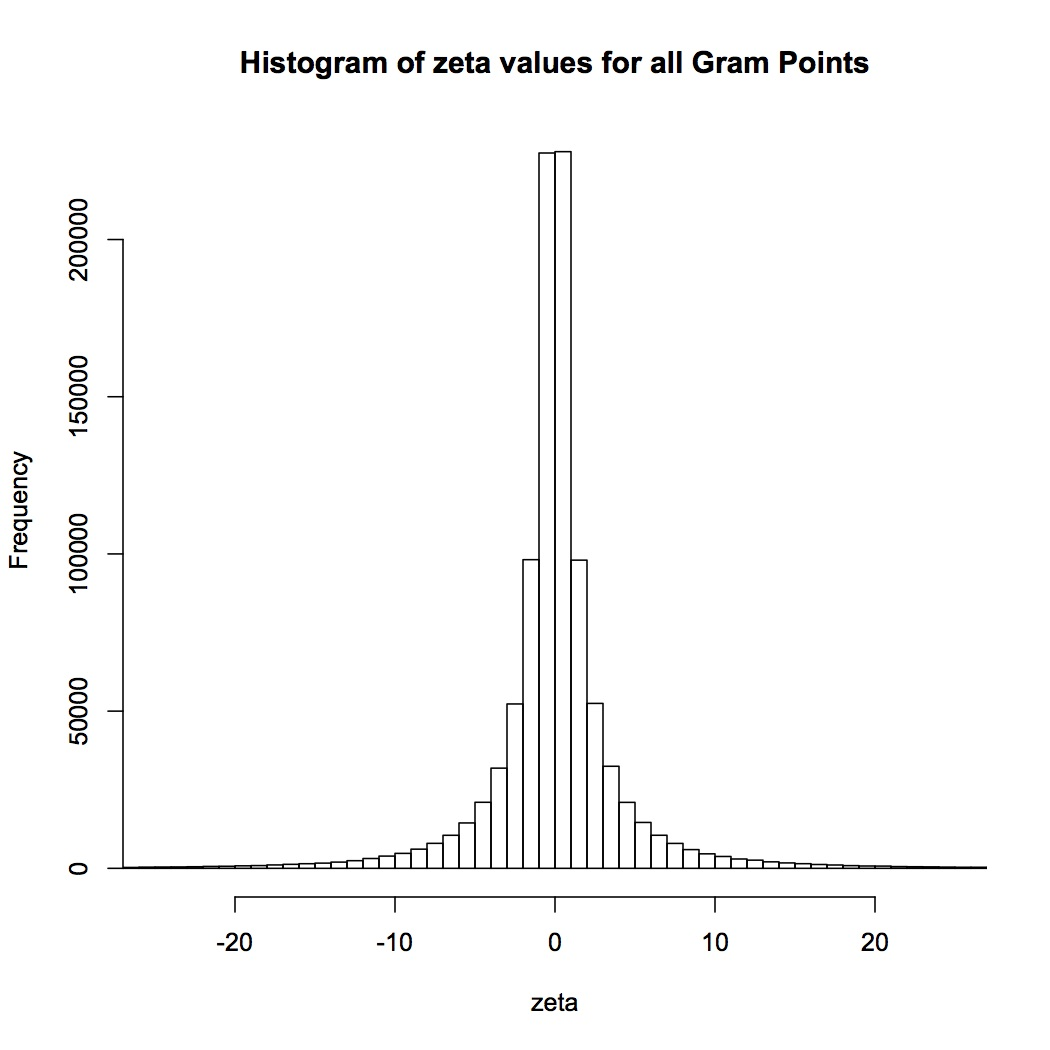
\includegraphics[width=0.8\textwidth]{rzeta.jpg}
\caption[]{ 
 Distribution of zeta values at a million Gram Points starting at $t = 10^{12}$.
  }
\label{ZeroDifferences}
\end{figure}

\begin{figure}
\centering
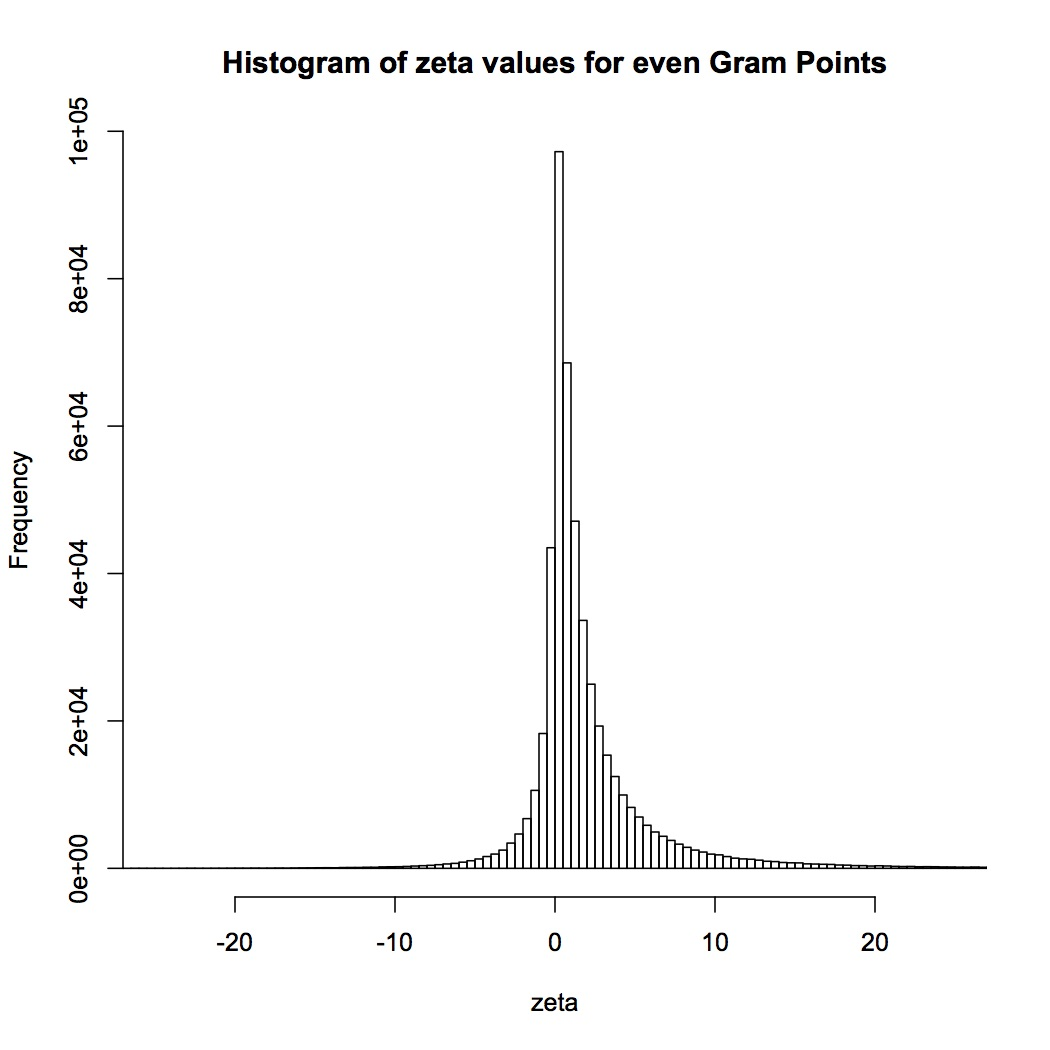
\includegraphics[width=0.8\textwidth]{ezeta.jpg}
\caption[]{ 
   Distribution of zeta values at 500000 even Gram Points starting at $t = 10^{12}$.
 }
\label{ZGram}
\end{figure}

\begin{figure}
\centering
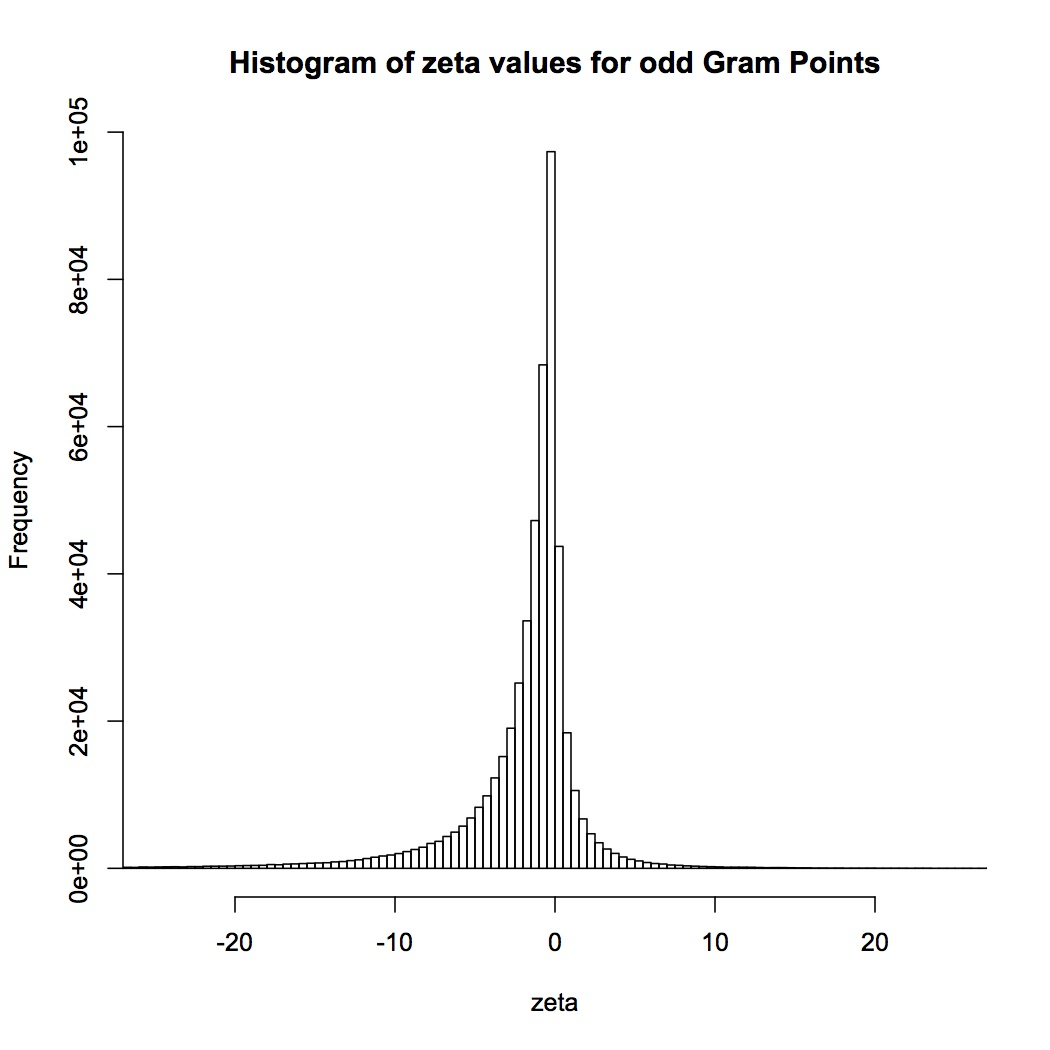
\includegraphics[width=0.8\textwidth]{ozeta.jpg}
\caption[]{ 
  Distribution of zeta values at 500000 odd Gram Points starting at $t = 10^{12}$.
 }
\label{NextZero}
\end{figure}


Reference to Conjecture \ref{antisymmetry}.
In this section we  establish the required notation for the 
Riemann Zeta Function. 
The Riemann Zeta function is defined for $\mathrm{Re} (s) > 1$ by
\begin{equation}
\zeta ( s ) \, = \, \sum^{\infty}_{n = 1} \; n^{-s} \, = \, \prod_{p \in primes} \;
\left( 1 - p^{-s} \right)^{-1}.
\label{eqRie}
\end{equation}

Eq.~(\ref{eqRie})  converges for $\mathrm{Re} (s) > 1$.  
 $\zeta ( s )$ has a  continuation
to the complex plane and satisfies a functional equation \cite{Riemann(1858),Riemann(1892),Titchmarsh(1986),Edwards(1974)}
\begin{equation}  
\xi(s):= \pi^{-s/2} \, \Gamma (s/2) \, \zeta ( s ) \, = \, \xi ( 1 - s );
\label{eq:func}
\end{equation}
$\xi(s)$ is entire except for simple poles at $s = 0$ and $1$. Riemann
multiplied the definition by $s(s-1)$ to remove the poles. We
write the zeroes of $\xi(s)$ as $1/2 + i \gamma$. The Riemann Hypothesis  
asserts that $\gamma$ is real for the non-trivial zeroes.
We order the $\gamma$s in increasing order, with 
\begin{equation}
\ldots \ldots \gamma_{-1} \, < \, 0 \, < \, 
\gamma_1 \, \leq \, \gamma_2 \ldots. 
\end{equation}
Then $\gamma_j \, = \, - \gamma_{-j}$ for $j = 1, 2, \ldots,$ 
and    $\gamma_1$, $\gamma_2$, $\ldots$  are roughly
$14.1347$, $21.0220$, $\ldots$.


Asymptotically, for the Riemann zeta function the mean number of 
zeros with height less than $\gamma$ (the smoothed Riemann zeta staircase)
is~\cite{Edwards(1974)}
\begin{equation}  
<\mathcal{N_R} (\gamma)> = (\gamma/2\pi)(ln(\gamma/2\pi)-1)-\frac{7}{8}.
\label{eq:Rnumber}
\end{equation}
Thus, the mean spacing of the zeros at height $\gamma$ is 
$2\pi(\ln (\gamma/2\pi))^{-1}$. For the range of $t$ values
studied by us this spacing is essentially constant at $0.2567$.

The study of the zeroes of the Riemann zeta function and Generalized 
Zeta functions is of interest to mathematicians and physicists. Mathematicians 
study the spacings because of its applications to analytic number theory, 
while physicists study it because of its  relation 
to the theory of the spectra of random matrix theories (RMT) 
and the spectra of classically chaotic quantum systems. 
Many remarkable properties of the Riemann zeta function keep turning up in the literature~\cite{os6,Matiyasevich}.


The next section gives the details of the numerical calculations.

\section{\label{sec3}Numerical Calculations}

In this section we discuss the details of the numerical work. 
The numerical analysis takes advantage of the functional 
equation Eq.~(\ref{eq:func}).
One defines
\begin{equation}
\theta(t) = arg (\pi^{−it/2} \Gamma(\frac{1}{4} + \frac{it}{2})), 
\label{eq:theta}
\end{equation}
where the argument is defined by continuous variation of $t$ starting with the value $0$ at $t = 0$.
For large $t$ $\theta$ has the asymptotic expansion
\begin{equation}
\theta(t) = \frac{t}{2}\ln (\frac{t}{2\pi}) - \frac{t}{2} - \frac{\pi}{8} + \frac{1}{48t} - \frac{1}{5760t^3}. 
\label{eq:thetaAsymptotic}
\end{equation}
A consequence of the zeta functional equation is that the function 
$Z(t)=exp(i\theta(t))\gamma(1/2 +it)$,
known as the Riemann-Siegel Z-function, is real valued for real $t$. 
Moreover we have $|Z(t)| = |\zeta(1/2+it)|$. Thus the zeros of $Z(t)$ are the imaginary part of the zeros 
of $\zeta(s)$ which lie on the critical line. We are led to finding the change of sign 
of a real valued function 
to find zeros on the critical line. This is a very convenient property in the numerical verification 
of the Riemann Hypothesis.
Another very helpful property is that many of the zeros are separated by the
"Gram points".  When $t \ge 7$, the $\theta$ function Eq.(\ref{eq:theta}) is monotonic increasing. 
For $n \ge 1$, the $n-th$ Gram point $g_n$ is defined as the unique solution $> 7$ to
$\theta (g_n) = n\pi$.
The Gram points are as dense as the zeros of $\zeta(s)$ but are much more regularly distributed.
Their locations can be found without any evaluations of the Riemann-Siegal series Eq.(\ref{eq:RS}).
Gram's law is the empirical observation that $Z(t)$ usually changes its sign in each Gram interval 
$G_n = [g_n,g_{n+1})$. 
This law fails infinitely often, but it is true in a large proportion of cases.
The average value of $Z(g_n)$ is $2$ for even $n$ and $-2$ for odd $n$~\cite{Titchmarsh(1986)},
and hence $Z(g_n)$ undergoes an infinite number of sign changes.
Figure~\ref{ZGram} shows the Riemann-Siegal function $Z(g_n)$ evaluated at 500 Gram points
starting at $n=99999999999$. Given the desirable properties of the Gram points, it seems 
natural to use the values at these points as the feature set for the neural network regression.


The Riemann-Siegel Z-function is evaluated using the Riemann-Siegal series
\begin{equation}
Z(t) = 2\sum^{m}_{n=1}\frac{\cos(\theta(t) - t \ln (n))}{\sqrt{n}} + R(t), 
\label{eq:RS}
\end{equation}
where $m$ is the integer part of $\sqrt{t/(2\pi)}$, and $R(t)$ is a small remainder
term which can be evaluated to the desired level of accuracy. The most important 
source for loss of accuracy at large heights is the cancellation between
large numbers that occur in the arguments of the $\cos$ terms in Eq.~(\ref{eq:RS}). We 
use a high precision module to evaluate the arguments. The rest of the calculation
is done using regular double precision accuracy. See ~\cite{hiary,gourdon,Odlyzko(1989)} for methods to
efficiently evaluate the zeta function at large t.
We calculated the zeta function at a million gram points starting at $t = 10^{12}$.

In the next section we discuss the application of neural network regression to aid
the location of the zeros. 


\begin{table}
\centering \(\begin{array}{c|c|c}
 Next~zero & Mean & Std. Deviation \\
\hline
Training~set \\
\hline
Acutal       & 0.579 & 0.41 \\
Predicted     & 0.579 & 0.37 \\
\hline
Validation~set \\
\hline
Acutal       & 0.599 & 0.42 \\
Predicted     & 0.590 & 0.38 \\
\hline
Test~set \\
\hline
Acutal       & 0.576& 0.43 \\
Predicted     & 0.581 & 0.39 \\

\end{array}\)
\caption{Prediction of the distance from a 
Gram point to the next zero.} \label{tab:nextZero}
\end{table}

\begin{table}
\centering \(\begin{array}{c|c|c}
Smallest~zero  & Mean & Std. Deviation \\
difference  &  &  \\
\hline
Training~set \\
\hline
Acutal       & 0.965 &  0.41 \\
Predicted     & 0.926 & 0.39 \\
\hline
Validation~set \\
\hline
Acutal       & 0.959 & 0.41 \\
Predicted     & 0.926 & 0.39 \\
\hline
Test~set \\
\hline
Acutal       & 0.972 & 0.43 \\
Predicted     & 0.934 & 0.42 \\

\end{array}\)
\caption{Prediction of the smallest zero difference in the Gram interval
with the left hand zero lying in the Gram interval.} \label{tab:zeroDiff}
\end{table}



\section{\label{conclusions}Conclusions}

xxx

\clearpage
 
\begin{thebibliography}{10} 

\bibitem{korolev1} Maxim Korolev,
"GRAM'S LAW AND THE ARGUMENT
OF THE RIEMANN ZETA FUNCTION", PUBLICATIONS DE L'INSTITUT MATH�MATIQUE,
\url{http://elib.mi.sanu.ac.rs/files/journals/publ/112/n106p053.pdf}, (2012)

\bibitem{korolev2} Maxim Korolev,
"On small values of the Riemann zeta-function at Gram points", Sbornik: Mathematics,
\url{http://iopscience.iop.org/article/10.1070/SM2014v205n01ABEH004367/meta},
{\bf205}, (2014)

\bibitem {Riemann(1858)} B. Riemann, ``\"{U}ber die Anzahl der Primzahlen uter
Einer Gegebenen Gr\"{o}be,'' {\it Montasb. der Berliner Akad.}, (1858),
671-680.

\bibitem {Riemann(1892)} B. Riemann, ``Gesammelte Werke'', Teubner, Leipzig, (1892).

\bibitem {Titchmarsh(1986)} E. Titchmarsh, ``The Theory of the Riemann Zeta
Function,'' Oxford University Press, Second Edition, (1986).

\bibitem {Edwards(1974)} H. M. Edwards, ``Riemann's Zeta Function,'' 
Academic Press,  (1974).

\bibitem{os6} O. Shanker, 
"Generalised Zeta Functions and Self-Similarity of Zero Distributions",
{\it J.  Phys. A} {\bf39}(2006), 13983-13997.

\bibitem {Matiyasevich} Y. Matiyasevich, 
"An artless method for calculating approximate values of
zeros of Riemann zeta function",
Web report, \url{http://logic.pdmi.ras.ru/~yumat/
personaljournal/artlessmethod/artlessmethodtexts.php}, (2013)

\bibitem{hiary} G. A. Hiary,
"METHODS TO COMPUTE THE RIEMANN ZETA
FUNCTION", arxiv.org, math.NT, 0711.5005v4, (2011).

\bibitem{gourdon} Xavier Gourdon,
"The $10^{13}$ first zeros of the Riemann Zeta function,
and zeros computation at very large height", report,
\url{http://numbers.computation.free.fr/Constants/Miscellaneous/zetazeros1e13-1e24.pdf}, (2004)

\bibitem {Odlyzko(1989)} A. Odlyzko, ``The $10^{20}$-th Zero of the Riemann Zeta
Function and 70 Million of its Neighbors,'' (preprint), A.T.T., (1989).

\end{thebibliography} 

\end{document} 

